% !TeX root = ../main.tex
% !TeX program = xelatex
% !TeX encoding = UTF-8
\section{多场景多尺度源荷协同优化方法}\label{minor:algorithm}

本节说明投资与运行的求解顺序、成本碳排权衡及结果检查方法。乌鲁木齐采用联合求解，固原和武汉采用锚定投资后的全季运行校核。算法总体流程如图\ref{fig:alg-overview}所示。

\begin{figure}[H]
\centering
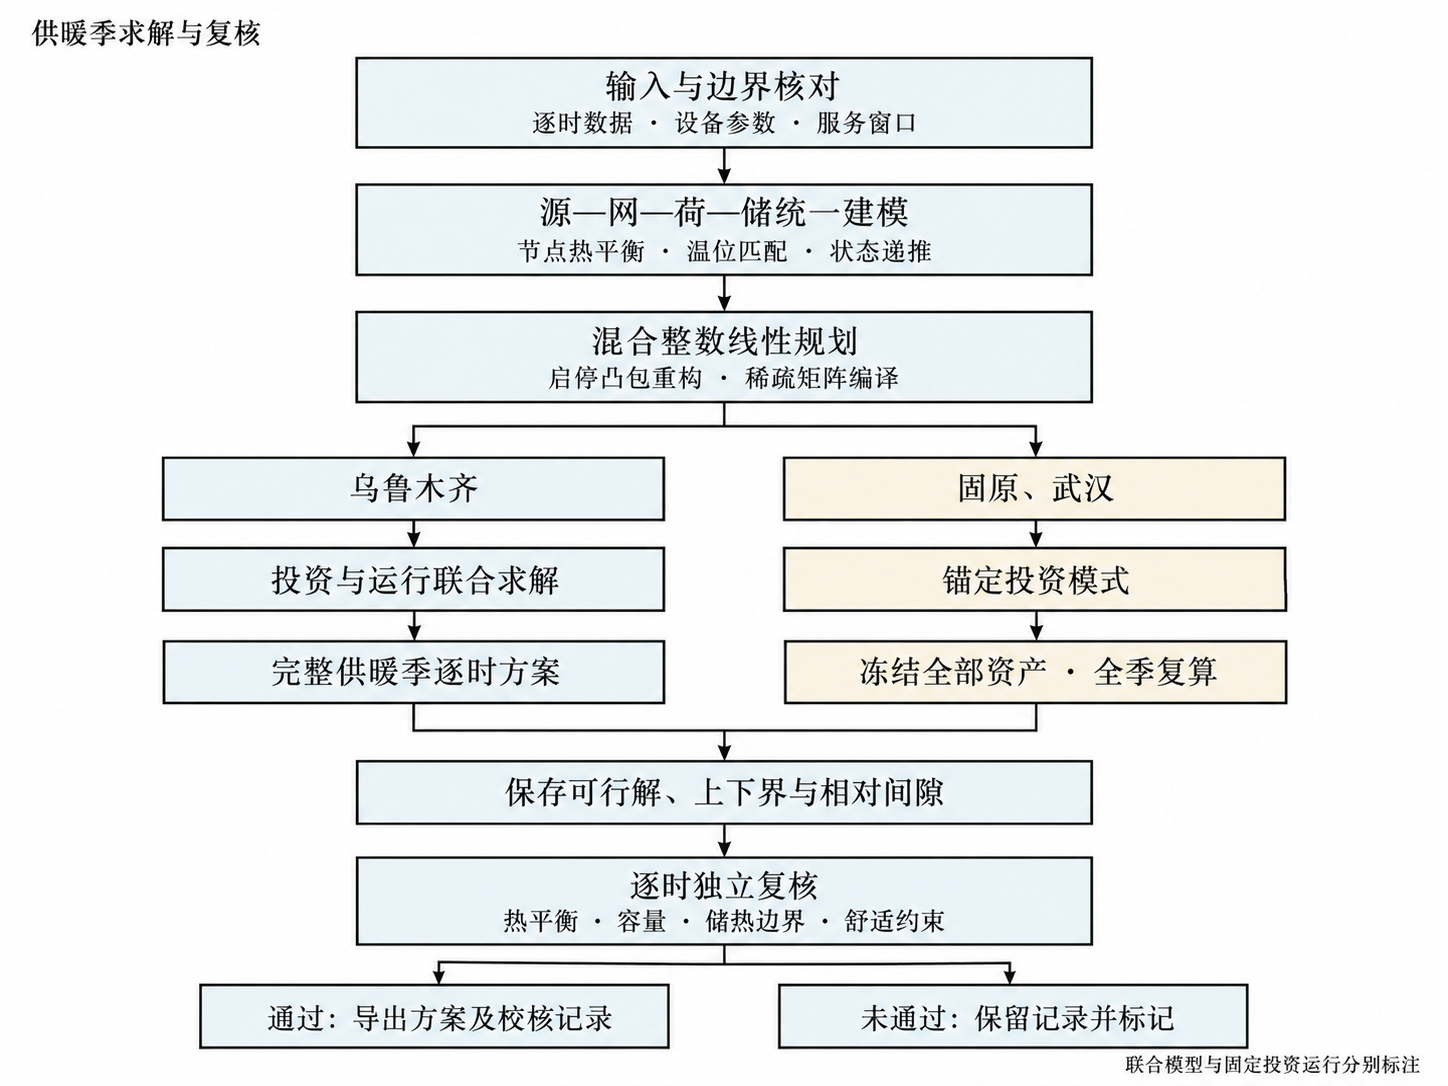
\includegraphics[width=\textwidth]{media/algorithm-revision/season_workflow_a2.png}
\caption{多尺度源荷协同优化算法总体流程}
\label{fig:alg-overview}
\end{figure}

\subsection{方法框架与可复现性}

算法输入包括逐时气象、分时电价、设备与财务参数、城市热网和建筑群画像；输出包括投资方案与逐时调度方案。投资变量涉及设备容量、温位模式、候选管径、储热规模、配电增容和用户侧改造，运行变量包括各热源出力、管网流量与温位、储热状态、需求响应量等。评价指标覆盖成本构成、碳排放、失供量、舒适度偏差和火用损失。

原始三城算例采用1~h时间步长，北京时间左闭右开：乌鲁木齐为2024年10月10日00:00至2025年4月11日00:00，固原为2024年10月15日00:00至2025年4月16日00:00，武汉为2024年11月16日00:00至2025年3月16日00:00，分别为4392~h、4392~h和2880~h。这些历史参数化仿真采用派生负荷及设备、费用假设，用于方法比较。每次求解均记录配置、输入数据指纹、求解状态和相对间隙，以形成可核验的计算记录。

与确定性单情景规划及工程手册式方案比选相比，本文算法的主要差异见表\ref{tab:alg-comparison}。

\begin{table}[H]
\centering
\caption{常见做法与本文算法的对照}
\label{tab:alg-comparison}
\begin{tabularx}{\textwidth}{L{0.27\textwidth}L{0.35\textwidth}Y}
\toprule
常见做法 & 本文算法 & 核验依据\\
\midrule
逐时离散化、确定性单情景规划 & 1~h全季求解，并开展多情景与极端年全年回放 & 主解求解记录、极端年累计61392~h回放\\
采用规划手册指标评价方案 & 单一MILP主解，并进行$\varepsilon$-约束与风险扫描 & 求解状态、上下界和相对间隙\\
规划与运行分开处理 & C1联合求解；C2、C3锚定投资后完成全季运行校核 & 投资层与运行层分别记录状态和间隙\\
\bottomrule
\end{tabularx}
\end{table}

\subsection{多尺度模型}

模型由城市层、区域层和用户层构成，各层通过共享投资变量、逐时运行变量和状态耦合约束连接。三个算例均采用3个模型节点，其中2个为聚合需求节点；乌鲁木齐、固原和武汉分别包含7、6、7类热源和3、2、1条聚合管段。城市层对应总体投资与技术路线，区域层对应热源和输配单元，用户层对应同类建筑负荷的聚合节点。其关系如图\ref{fig:alg-multiscale}所示。

\begin{figure}[H]
\centering
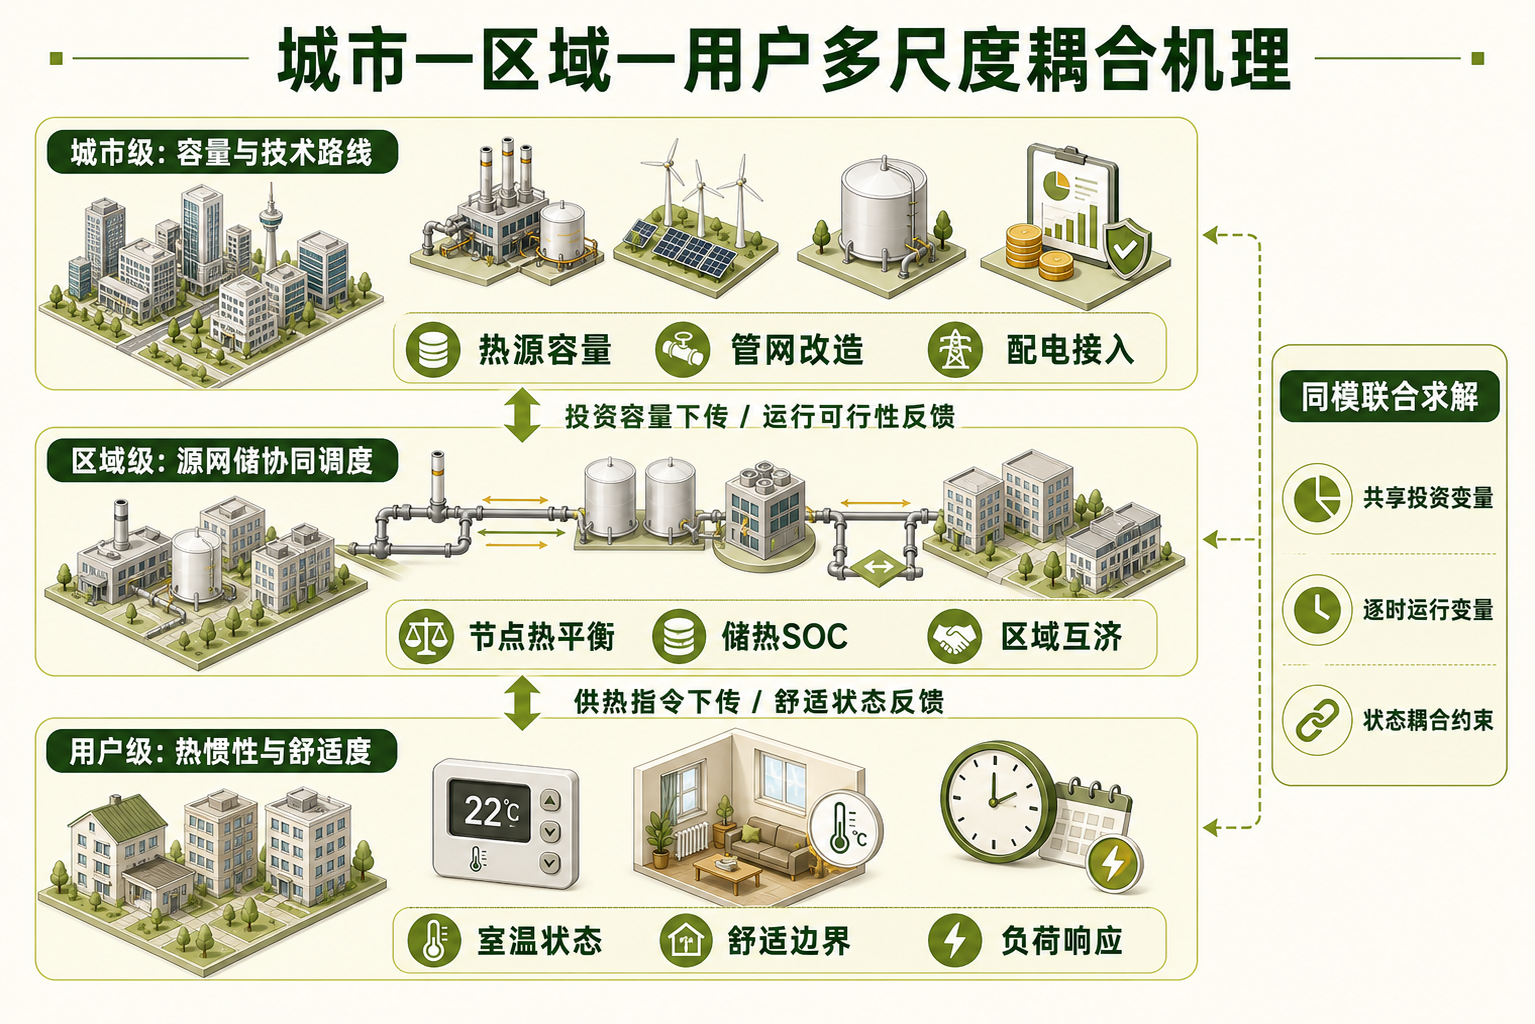
\includegraphics[width=0.76\textwidth,height=0.30\textheight,keepaspectratio]{media/algorithm-revision/fig2.png}
\caption{城市---区域---用户多尺度耦合机制}
\label{fig:alg-multiscale}
\end{figure}

城市层确定容量与技术路线，包括新增或退役机组容量、热源温位模式、候选管径、储热规模以及配电接入和增容。候选技术链依据资源、场地、配电和政策条件生成并预筛，本次计算执行容量、拓扑和温级预审。

区域层描述能流、管网与储热。模型在节点和75/45~$^{\circ}$C两级温位上建立逐时能量平衡。温位兼容约束阻止低温热源直接供应高温需求，高温热源供应低温需求时将品位损失计入火用失配惩罚：
\begin{equation}
T_{\mathrm{src}}^{\min}\geq T_{\mathrm{sup}}+\Delta T_{\mathrm{he}},
\label{eq:alg-grade}
\end{equation}
该不等式用于已选直接供热路径。其中，$T_{\mathrm{src}}^{\min}$为热源供水温度下界，$T_{\mathrm{sup}}$为用户供水温度要求，$\Delta T_{\mathrm{he}}$为换热端差。管网采用温位线性化和双向流动互斥约束，储热状态按下式递推：
\begin{equation}
E_{s,t}=(1-\mu_s)E_{s,t-1}+\eta_{\mathrm{ch}}q_{s,t}^{\mathrm{ch}}\Delta t-\frac{q_{s,t}^{\mathrm{dis}}\Delta t}{\eta_{\mathrm{dis}}},
\label{eq:alg-storage}
\end{equation}
其中，$\mu_s$为自损失率，$\eta_{\mathrm{ch}}$和$\eta_{\mathrm{dis}}$分别为充、放热效率。

用户层描述聚合节点的热惯性与负荷调节。原聚合算例采用前节的单一等效热状态；新增逐楼验证采用精确离散1R1C模型。状态上下界、需求响应窗口守恒和参与率上限共同约束聚合用户侧调节行为。等效热状态递推为
\begin{equation}
E_{n,t}=(1-\lambda_n)E_{n,t-1}+(q_{n,t}^{+}-q_{n,t}^{-})\Delta t,
\qquad \Delta\theta_{n,t}=E_{n,t}/C_n,
\label{eq:alg-building}
\end{equation}
其中，$C_n$为节点$n$的等效热容，$q^+_{n,t}$和$q^-_{n,t}$为相对基准负荷的增加与削减功率。逐楼模型保留供热变化引起的散热变化，按对应算例单独验证。

三个尺度通过容量、温位和建筑改造三类接口耦合：容量约束将运行出力限制在可用率及设备上下限内；温位矩阵完成“源温---网温---节点负荷”匹配；用户侧调节量先进入节点热平衡，再由热源出力与储热充放共同响应。例如在已有逐时结果中，用户侧负荷削减使同一时段节点需求下降，优先减少边际热源出力；恢复负荷出现时，由储热与可调热源按相应解共同响应，节点平衡在每个时段保持闭合。乌鲁木齐场景采用投资---运行联合MILP；固原和武汉因问题规模采用锚定两阶段方法，先确定投资模式，再冻结投资开展全季运行校核。因此，后两个场景的推荐方案用于工程可行性比较，不将投资层结果表述为全局最优。

\subsection{多目标协同优化}\label{minor:multiobjective}

成本与碳排放采用$\varepsilon$-约束法协调\supcite{32}。费用目标仍保留场景配置的碳价和偏好项；仅专用无碳价入口以基本费用形成比较。模型以全生命周期净成本的等年值最小为目标，同时设置碳排放上限；逐档收紧上限并重新求解完整供暖季，相邻两档的成本增量与减排量之比用于计算边际减排成本。

乌鲁木齐场景中，成本端点为27.49万元、27.32~t~CO$_2$，排放端点为74.81万元、10.57~t~CO$_2$。本文推荐记录采用通过该记录已启用硬约束与校核的方案，等年值成本为27.76万元、碳排放为27.31~t~CO$_2$；该记录与仅按目标函数排序得到的成本端点分开标注。单位供热成本由基准方案的0.078851元/kWh增至0.100681元/kWh，增加27.69\%。该增幅反映以成本增加换取减排、清洁热利用和可靠性约束的综合取舍。

零失供、清洁热比例、N$-1$容量裕度及对应热状态上下限按已启用配置作为硬边界，不与经济性目标交换；地源年度平衡保留为可选约束。失供率约束为
\begin{equation}
U_{\mathrm{un}}=\frac{\sum_t q_t^{\mathrm{un}}}{\sum_t Q_t}\leq U_{\max},
\label{eq:alg-unserved}
\end{equation}
其中，$q_t^{\mathrm{un}}$为失供功率，$Q_t$为热需求，$U_{\max}=0$表示推荐方案不允许失供。边界内的需求移峰和舒适偏差通过惩罚成本进行优化。

气象不确定性作为独立风险层，采用
\begin{equation}
\min\ \mathbb{E}[C]+\lambda\operatorname{CVaR}_{\alpha}(C),
\qquad \alpha=0.8,
\label{eq:alg-risk-objective}
\end{equation}
其中，$\lambda$取0、0.02、0.05和0.10四档。条件风险价值采用Rockafellar--Uryasev线性化：
\begin{equation}
\operatorname{CVaR}_{\alpha}(C)=\min_{\eta,z_s}\left\{\eta+\frac{1}{1-\alpha}\sum_s p_sz_s\right\},
\quad z_s\geq C_s-\eta,\quad z_s\geq0.
\label{eq:alg-cvar}
\end{equation}

$\lambda=0.05$作为三个场景的统一参考值。多气象年风险层中，乌鲁木齐的期望成本增加0.012万元、CVaR下降0.831万元；固原的期望成本增加0.016万元、CVaR下降0.515万元，变化约占年化成本的0.01\%。武汉场景的投资不随风险权重改变，说明其投资方案主要由硬约束决定。不同风险权重下的结构变化见表\ref{tab:alg-lambda}。

\begin{table}[H]
\centering
\caption{多气象年风险层的$\lambda$权重扫描结果}
\label{tab:alg-lambda}
\begin{tabularx}{\textwidth}{cYYY}
\toprule
$\lambda$ & 乌鲁木齐 & 固原 & 武汉\\
\midrule
0.02 & 余热源热泵、备用电锅炉和配电容量首次调整 & 投资配置不变 & 投资配置不变\\
0.05 & 继续小幅调整 & 储热与微网可再生增加，生物质调峰减少 & 投资配置不变\\
0.10 & 进一步转入风险平衡 & 与0.05档接近 & 投资配置不变\\
\bottomrule
\end{tabularx}
\end{table}

$\lambda$扫描来自2020---2024多气象年全年回放，用于风险机制专项验证；供暖季主结果中的成本---碳Pareto采用确定性单情景计算。风险层共包含12个规划案例（3个场景$\times$4档$\lambda$），全部收敛，60项年度容量审计通过，CVaR台账一致性误差为$5.59\times10^{-9}$元。图\ref{fig:alg-objectives}展示的是该专项风险层的12/12案例收敛与60/60容量审计结果，不等同于供暖季推荐方案的13道机器验收。

\begin{figure}[H]
\centering
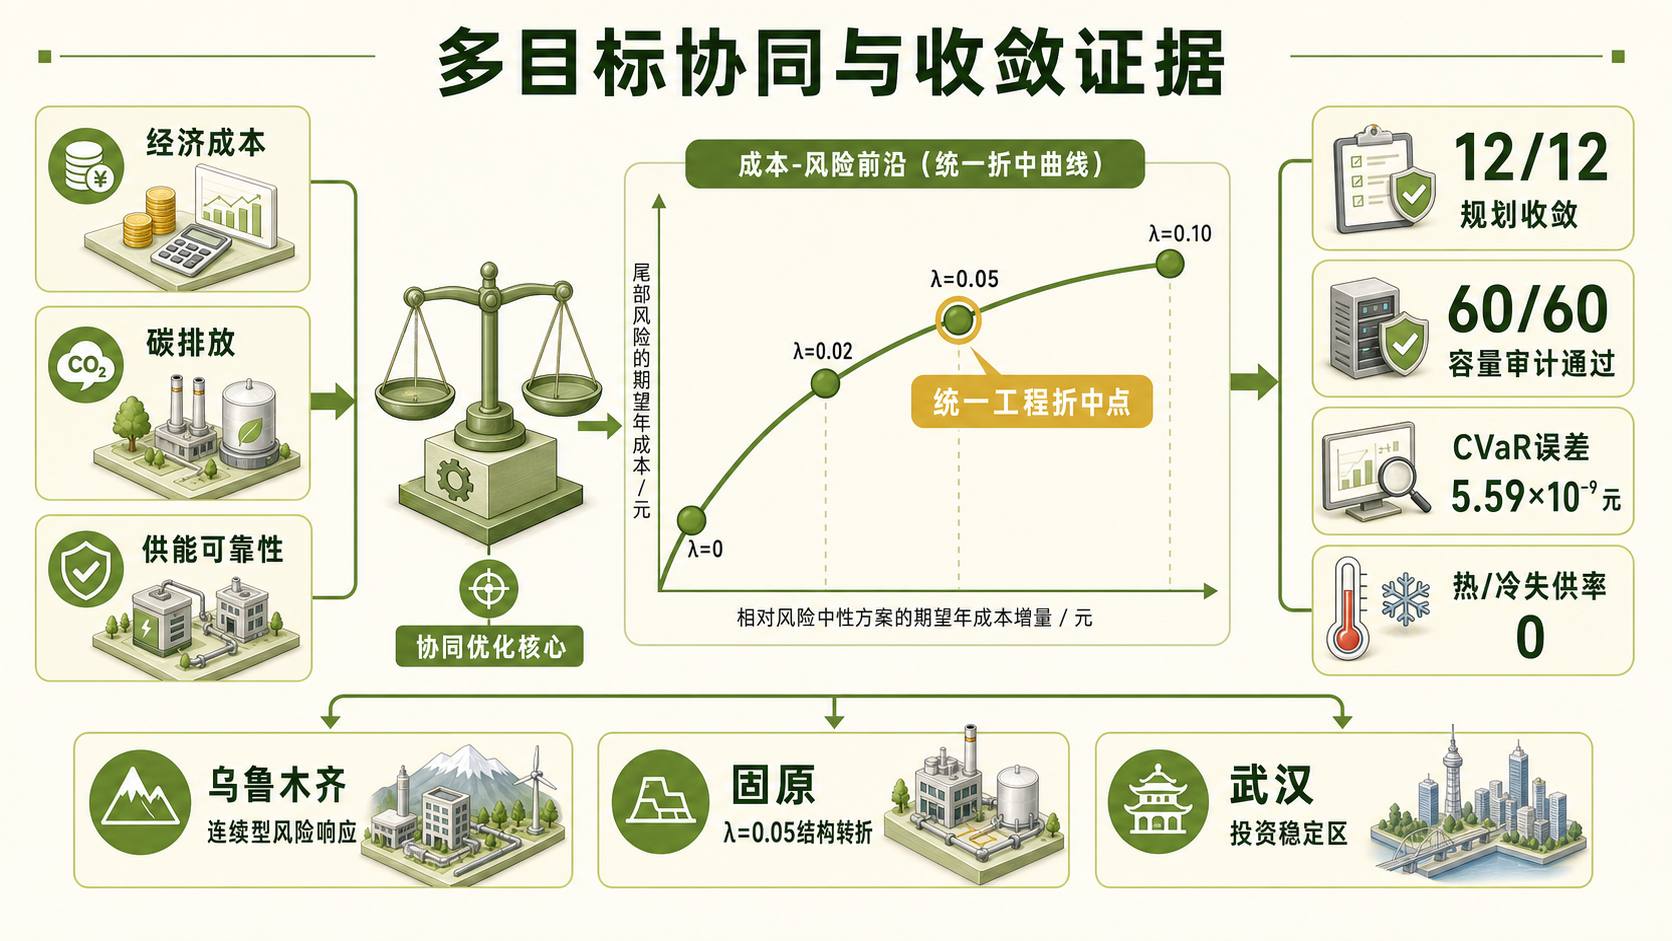
\includegraphics[width=0.76\textwidth,height=0.30\textheight,keepaspectratio]{media/algorithm-revision/fig3.png}
\caption{多目标协同与风险层收敛证据}
\label{fig:alg-objectives}
\end{figure}

\subsection{求解流程与收敛准则}

模型构造器采用Python~3.11实现，并通过SciPy的\texttt{milp}接口调用HiGHS求解。约束矩阵按CSR/CSC稀疏格式编译和缓存，模型装配约需1.6~s，未使用自定义割。机组启停采用凸包重建模，开机状态保留为二元变量，启动和停机辅助变量连续化。全年回放单城测试中，整数变量数量由26280个减至8760个。

算法\ref{alg:season-workflow}给出主结果的求解与校核顺序，算法\ref{alg:epsilon-workflow}给出独立碳帽扫描。优化器一次求解整个声明窗口，小时索引用于建立守恒与状态约束。求解状态、相对间隙、约束残差和后验校核分别登记；时限内可行解保留其近似解身份。附录3列出与这些步骤对应的真实Python代码节选。

% !TeX root = ../main.tex
\newcounter{paperalgorithm}
\newenvironment{paperalgorithm}[2]{%
  \par\Needspace{15\baselineskip}\refstepcounter{paperalgorithm}\label{#2}%
  \begingroup\small\setstretch{1.05}\setlength{\parskip}{4pt}%
  \noindent\rule{\linewidth}{0.6pt}\par\noindent\textbf{算法\thepaperalgorithm\quad #1}\par
}{\par\noindent\rule{\linewidth}{0.6pt}\par\endgroup}

\begin{paperalgorithm}{供暖季求解与复核流程}{alg:season-workflow}
\noindent\textbf{输入：}场景配置、规划输入、连续供暖季逐时数据和求解容差。\par
\noindent\textbf{输出：}投资及逐时运行方案，求解状态、间隙和校核记录。
\begin{enumerate}[label=\arabic*.,leftmargin=1.8em,itemsep=2pt,topsep=3pt,parsep=0pt]
\item 核对时间范围、步长、缺测及单位；读取各模块启用状态与参数来源。
\item 装配源、网、荷、储及电力接口；对所有小时联立守恒、容量和热状态约束，设置初始及期末边界。
\item \textbf{若采用联合求解：}在完整声明窗口同时求投资与运行方案。
\item \textbf{若采用固定投资复算：}求得规划方案或读入已登记方案；将全部投资项冻结为存量，保持可靠性条件，再构造全季运行模型并求解。
\item 保存可行解、求解状态、上下界及相对间隙；无可行解时随异常报告失败原因，结束本次计算。
\item 按实际启用模块，复核逐时平衡、容量、储热边界、舒适约束与服务期覆盖；校核不通过则保留记录并标记未通过。
\item 导出配置、投资、逐时运行与检查结果；分别标注联合模型可行解或固定投资下可行解。
\end{enumerate}
\end{paperalgorithm}

\begin{paperalgorithm}{独立费用—碳排放采样接口}{alg:epsilon-workflow}
\noindent\textbf{输入：}同一配置和时间序列、碳帽档数$K\geq2$。\par
\noindent\textbf{输出：}通过复核的采样非支配方案、边际减排费用和折中建议。
\begin{enumerate}[label=\arabic*.,leftmargin=1.8em,itemsep=2pt,topsep=3pt,parsep=0pt]
\item 复制输入配置，清除原碳帽并令碳价为零；保留设备、运行与可靠性约束。
\item 分别以费用和排放为主目标求端点；第二阶段约束主目标不高于第一阶段可行值加容差，再优化次目标。
\item 检查端点排放的先后关系；不满足容差要求则终止，满足时在两端排放值间等距设置$K$档碳帽。
\item \textbf{对每档碳帽：}复制同一基础配置，加数值容差后施加碳帽；按费用目标重新构模并求解。投资项是否固定取决于输入配置。
\item 对本档解独立检查数值残差和碳帽；任一检查不通过则报错并终止扫描，通过则保存全部结果。
\item 对通过的样本去重并剔除受支配点，计算相邻方案的边际减排费用；用归一化理想点距离给出折中建议。
\end{enumerate}
\end{paperalgorithm}

算法\ref{alg:epsilon-workflow}对应当前代码的独立接口，流程见图\ref{fig:epsilon-workflow-a2}。所得集合限于已采样可行解，折中建议取决于归一化规则。供暖季历史扫描保留其原记录中的碳价与偏好，不与这一接口混记。

\begin{figure}[H]
\centering
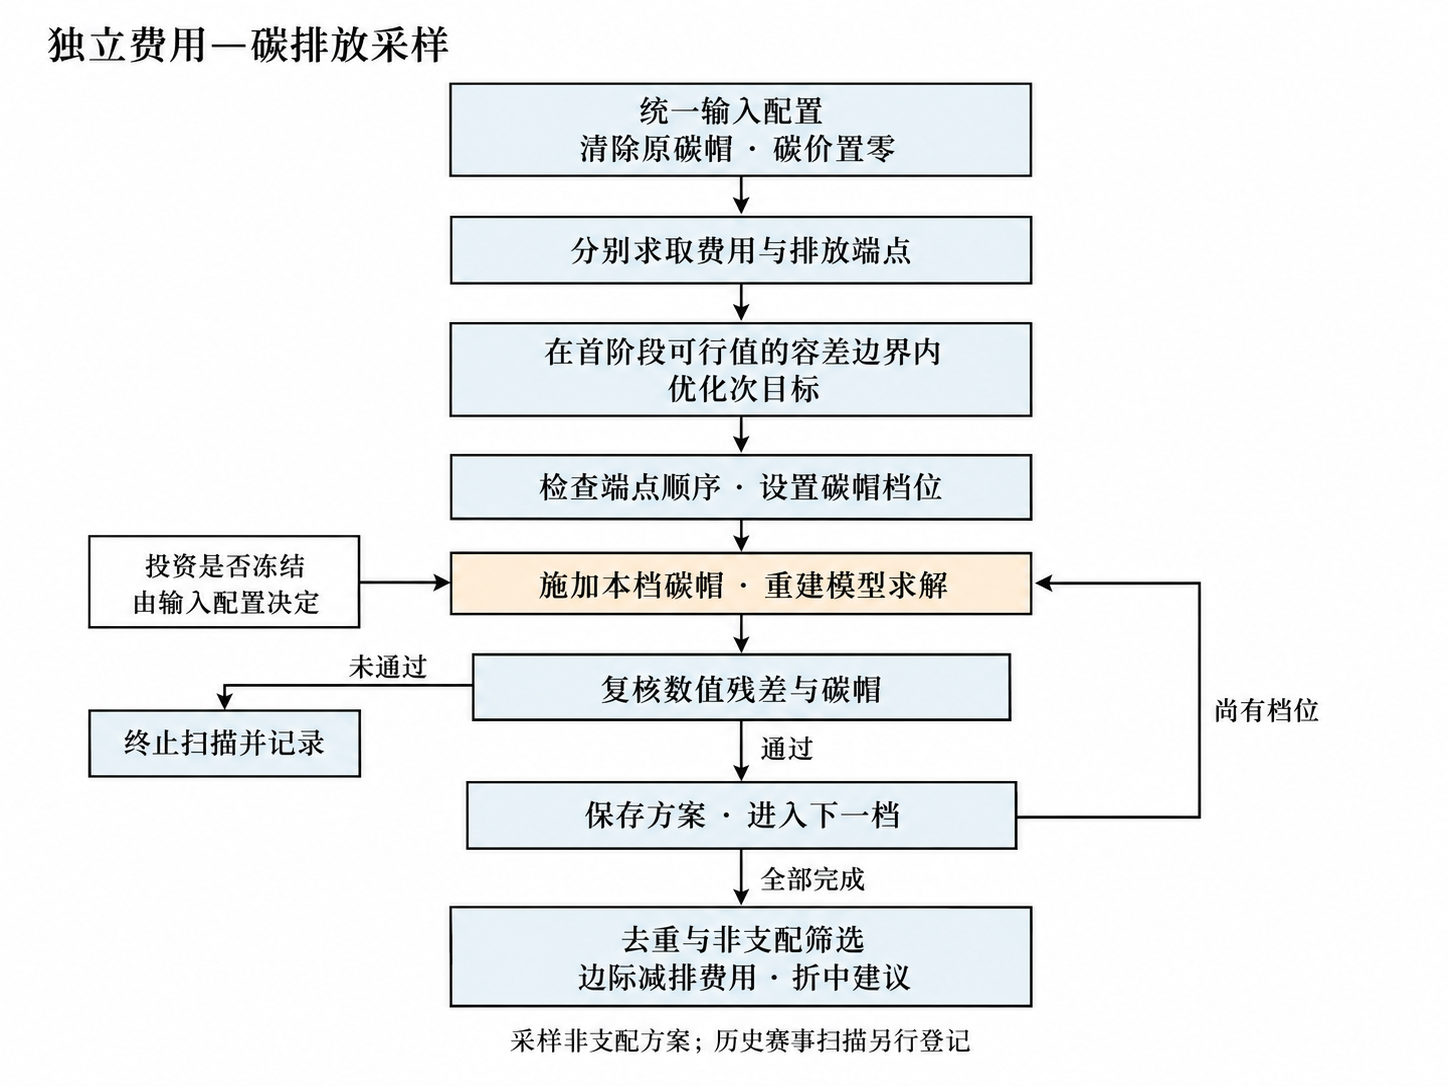
\includegraphics[width=\textwidth]{media/algorithm-revision/epsilon_workflow_a2.png}
\caption{独立费用---碳排放采样与复核流程}
\label{fig:epsilon-workflow-a2}
\end{figure}


乌鲁木齐联合模型的相对间隙为$1.53\times10^{-4}$；固原锚定投资后的运行层间隙为$1.84\times10^{-3}$；武汉运行层为连续规划，间隙为0，其投资层记录为0.98\%。三场景逐时热平衡最大绝对残差依次为$7.41\times10^{-13}$、$1.25\times10^{-10}$和$8.53\times10^{-14}$~kW，均低于$10^{-6}$~kW容差。投资层、运行层与机器验收分别留存状态，不将固原和武汉表述为联合求解通过。结果见表\ref{tab:alg-solver}。

\begin{table}[H]
\centering
\caption{三场景推荐方案求解与验收结果}
\label{tab:alg-solver}
\small
\begin{tabularx}{\textwidth}{@{}L{0.11\textwidth}L{0.20\textwidth}L{0.18\textwidth}L{0.09\textwidth}L{0.14\textwidth}Y@{}}
\toprule
场景 & 求解方法 & 整数变量 & 时间/s & 相对间隙/\% & 结果属性\\
\midrule
乌鲁木齐 & 投资---运行联合MILP & 启停二元8784个 & 531.1 & 联合层0.0153 & 联合模型可行解\\
固原 & 锚定两阶段 & 运行层启停二元4392个 & 64.0 & 运行层0.184 & 固定投资下可行解\\
武汉 & 锚定投资+连续运行 & 0 & 31.7 & 运行层0；投资层0.98 & 固定投资下可行解\\
\bottomrule
\end{tabularx}
\end{table}

敏感性测试的20档扰动获得有效解，其中乌鲁木齐电价高档和余热低档为时间受限近似解，相对间隙分别为7.05\%和9.44\%；另有固原负荷低档、武汉碳价高档两档未收敛。乌鲁木齐Pareto中间档的部分点在时限内间隙为13.2\%---13.7\%。固原三档采用推荐投资模式复算，全部满足碳排放上限，间隙为0.20\%、0.22\%和0.24\%，这些结果属于冻结投资模式的运行参考点，不代表完整联合MILP重新寻优。

为检验乌鲁木齐排放端点投资模式在不同碳帽下的运行可达性，固定排放端点记录的投资、退役、管径、储热和末端改造模式，对23365、19136和14906~kg三档碳帽进行全季运行重算。三档实际排放均为10616.5~kg，失供率为0，求解状态均为Optimal，相对间隙为$1.90\times10^{-7}$。运行成本为11.271万元/年，仅包含运行费用，不与联合解中包含资本成本的Pareto结果直接比较。

\subsection{计算效率与扩展性}

求解效率的改善主要来自启停凸包重建模和稀疏编译缓存。固原全年回放用时由575.746~s降至86.903~s，提升6.63倍；两年度合计用时由602.483~s降至112.750~s，减少81.29\%。该结果来自多气象年全年回放的单城效率测试。单次供暖季问题约包含31万---45万个变量，乌鲁木齐场景的启停二元变量为8784个。连续温位、C\&CG、Benders分解和在线MPC作为可选扩展，本次计算未启用。逐时回放、边界检验和求解加速关系如图\ref{fig:alg-replay}所示。

\begin{figure}[H]
\centering
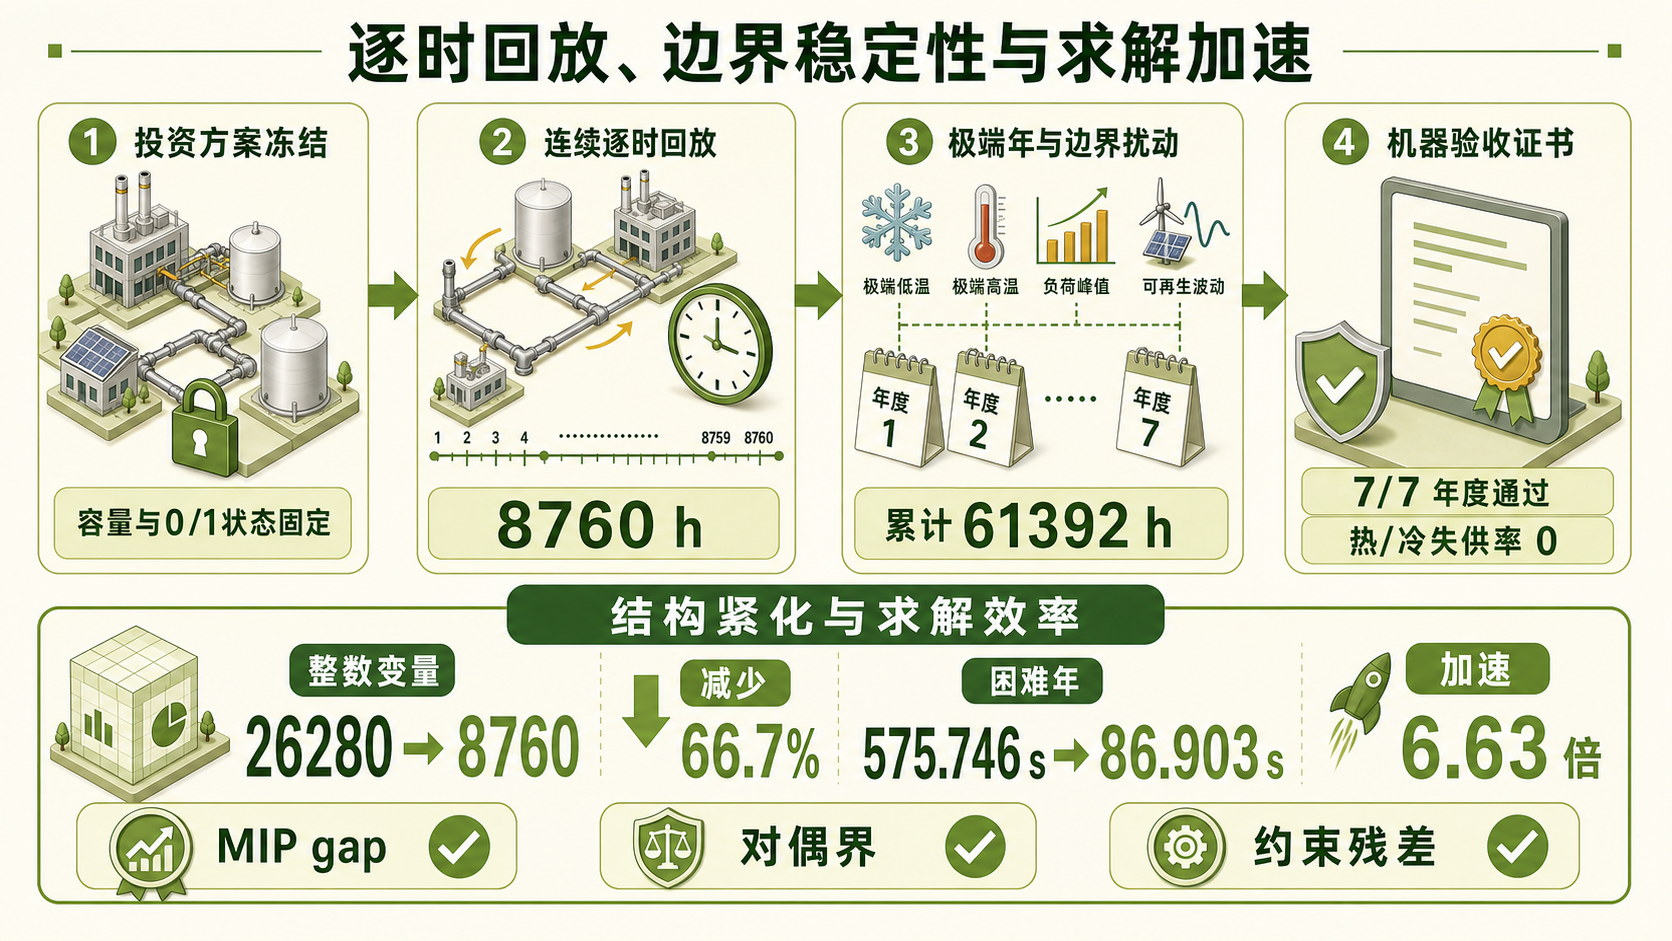
\includegraphics[width=0.76\textwidth,height=0.30\textheight,keepaspectratio]{media/algorithm-revision/fig4.png}
\caption{逐时回放、边界稳定性与求解效率}
\label{fig:alg-replay}
\end{figure}

\subsection{数值结果与敏感性}

图\ref{fig:code-kpi}比较了基准方案与推荐方案的成本、碳排放、清洁热利用和供热可靠性指标。推荐方案的取舍由成本、排放上限、清洁热占比和供热约束共同决定，因此各项指标的变化方向并不完全一致。图中成本采用年化等效口径，单位供热成本按交付热量折算，二者与供暖季现金运行成本分别核算。

\begin{figure}[H]
\centering
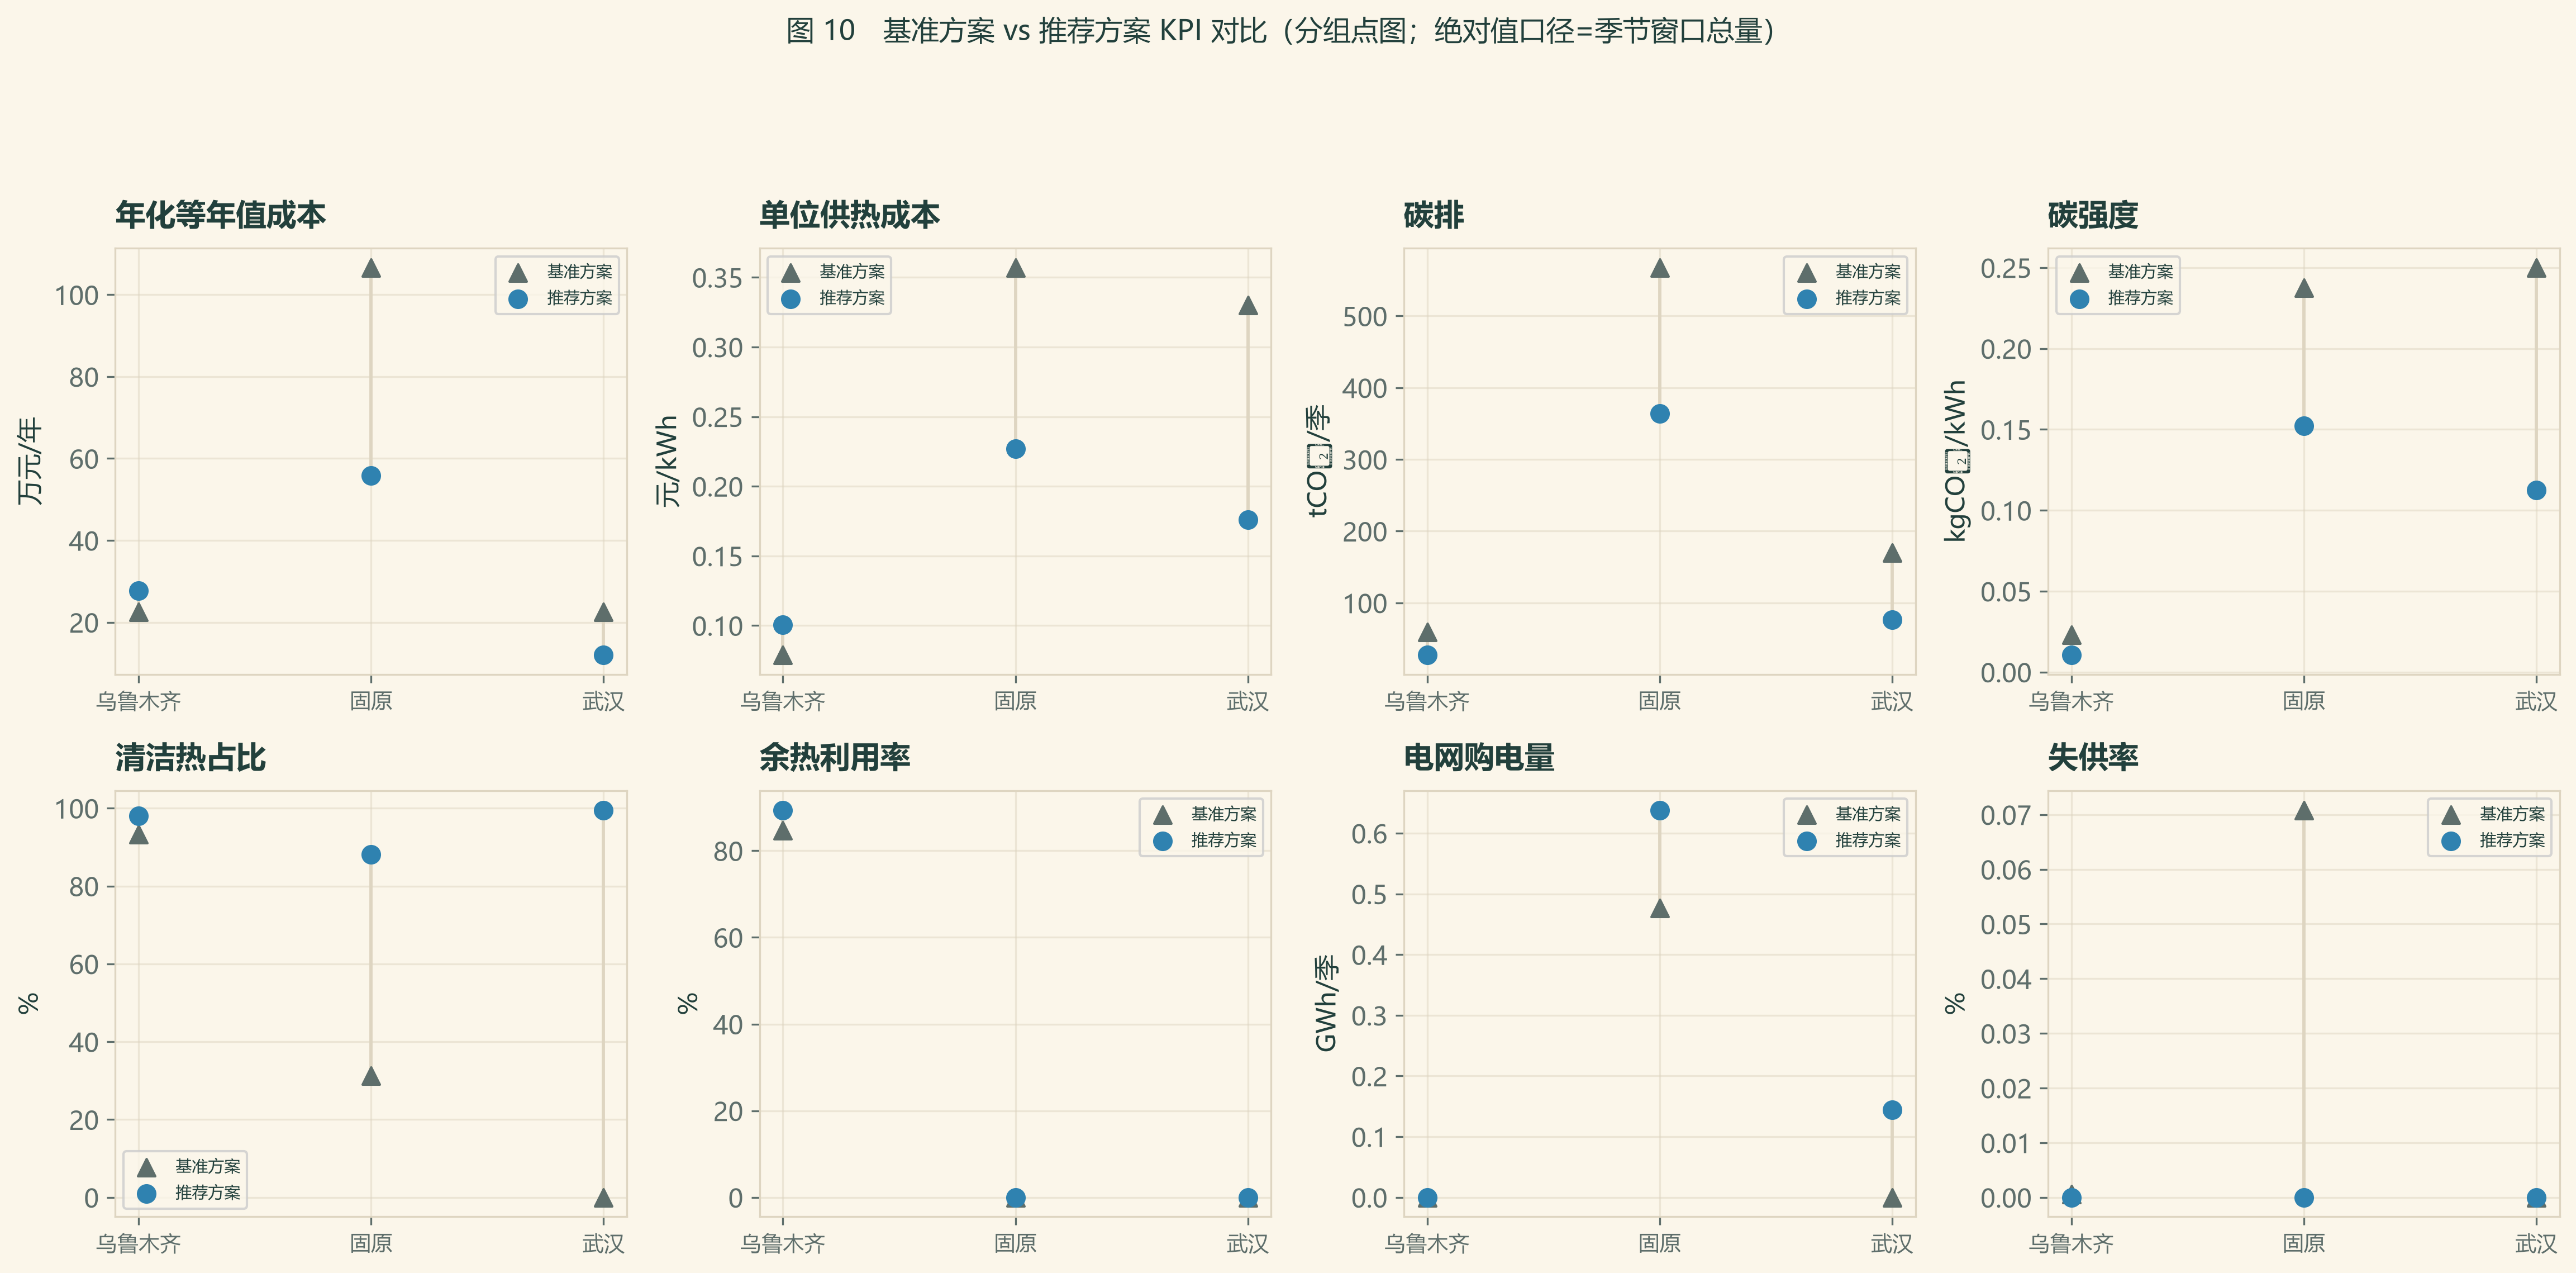
\includegraphics[width=0.98\textwidth,height=0.52\textheight,keepaspectratio,trim=0 0 0 100,clip]{media/code-results/fig10_kpi_comparison.png}
\caption{基准方案与推荐方案KPI对比}
\label{fig:code-kpi}
\end{figure}

成本与碳排放的候选解分布见图\ref{fig:code-pareto}。推荐方案从满足排放、可靠性和投资边界的候选解中选取，不必与最低成本点或最低排放点重合。部分点为固定投资模式下的运行参考点或时限内近似解，其求解状态和相对间隙以前文说明为准。

\begin{figure}[H]
\centering
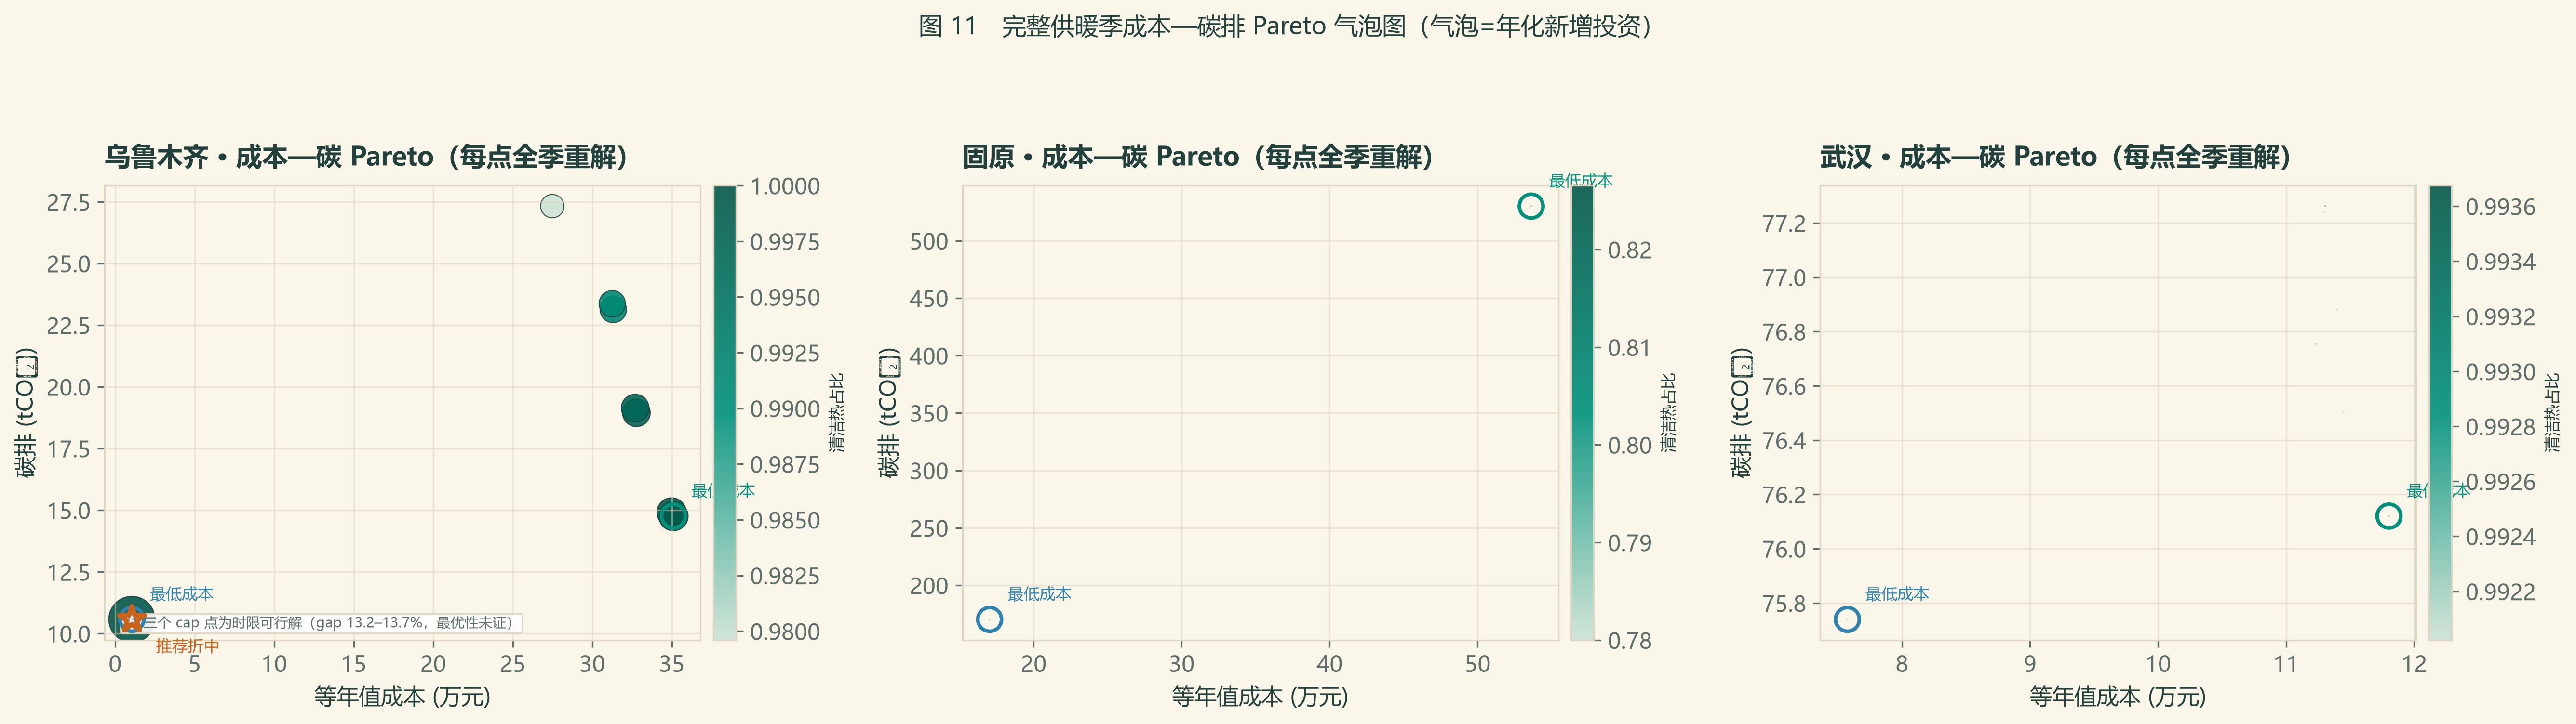
\includegraphics[width=0.78\textwidth,height=0.33\textheight,keepaspectratio,trim=0 0 0 100,clip]{media/code-results/fig11_cost_emission_pareto.png}
\caption{三城市成本—碳排放候选方案对比}
\label{fig:code-pareto}
\end{figure}

V4全年单情景消融实验沿用原时间权重，并在每次移除模块后重新求解投资与运行。完整模型的年化目标为95.620万元，碳排放为30.602万kg~CO$_2$。去掉需求响应后，年化成本增加0.09\%，购电量增加0.21\%；去掉新增储热后，年化成本增加3.55\%，碳排放增加6.05\%，购电量增加3.41\%；去掉火用失配惩罚后，火用损失增加4.90\%。该组结果用于检验V4模块贡献，与三城市供暖季推荐方案分开报告。

复合寒潮压力测试沿用V4算例，将室外温度序列整体降低8~$^{\circ}$C、负荷提高15\%、余热可用量降低15\%，并冻结投资变量。测试结果仍保持零失供；按同一能源运行费口径，费用由50.057万元增至100.349万元，增加100.47\%，购电量增加56.78\%，碳排放增加113.95\%。逐档敏感性分析表明：乌鲁木齐对热负荷最敏感，成本变化为$+19.1\%/-17.9\%$，其次为余热下降和电价上升；固原的生物质到货扰动因库存缓冲未改变成本；武汉对电价和热负荷较敏感，变化范围分别为$+16.9\%/-14.6\%$和$+16.8\%/-13.7\%$。

最冷连续168~h的热源出力、负荷和储热状态见图\ref{fig:code-cold168}，用于检查低温持续期间的逐时供需平衡。图\ref{fig:code-worst72}进一步列出最不利72~h窗口内的可用供热能力、负荷、储热与容量裕度。两图分别反映常规极寒时段调度和压力场景下的边界状态，不据此假定三城市具有相同的储热运行模式。

\begin{figure}[H]
\centering
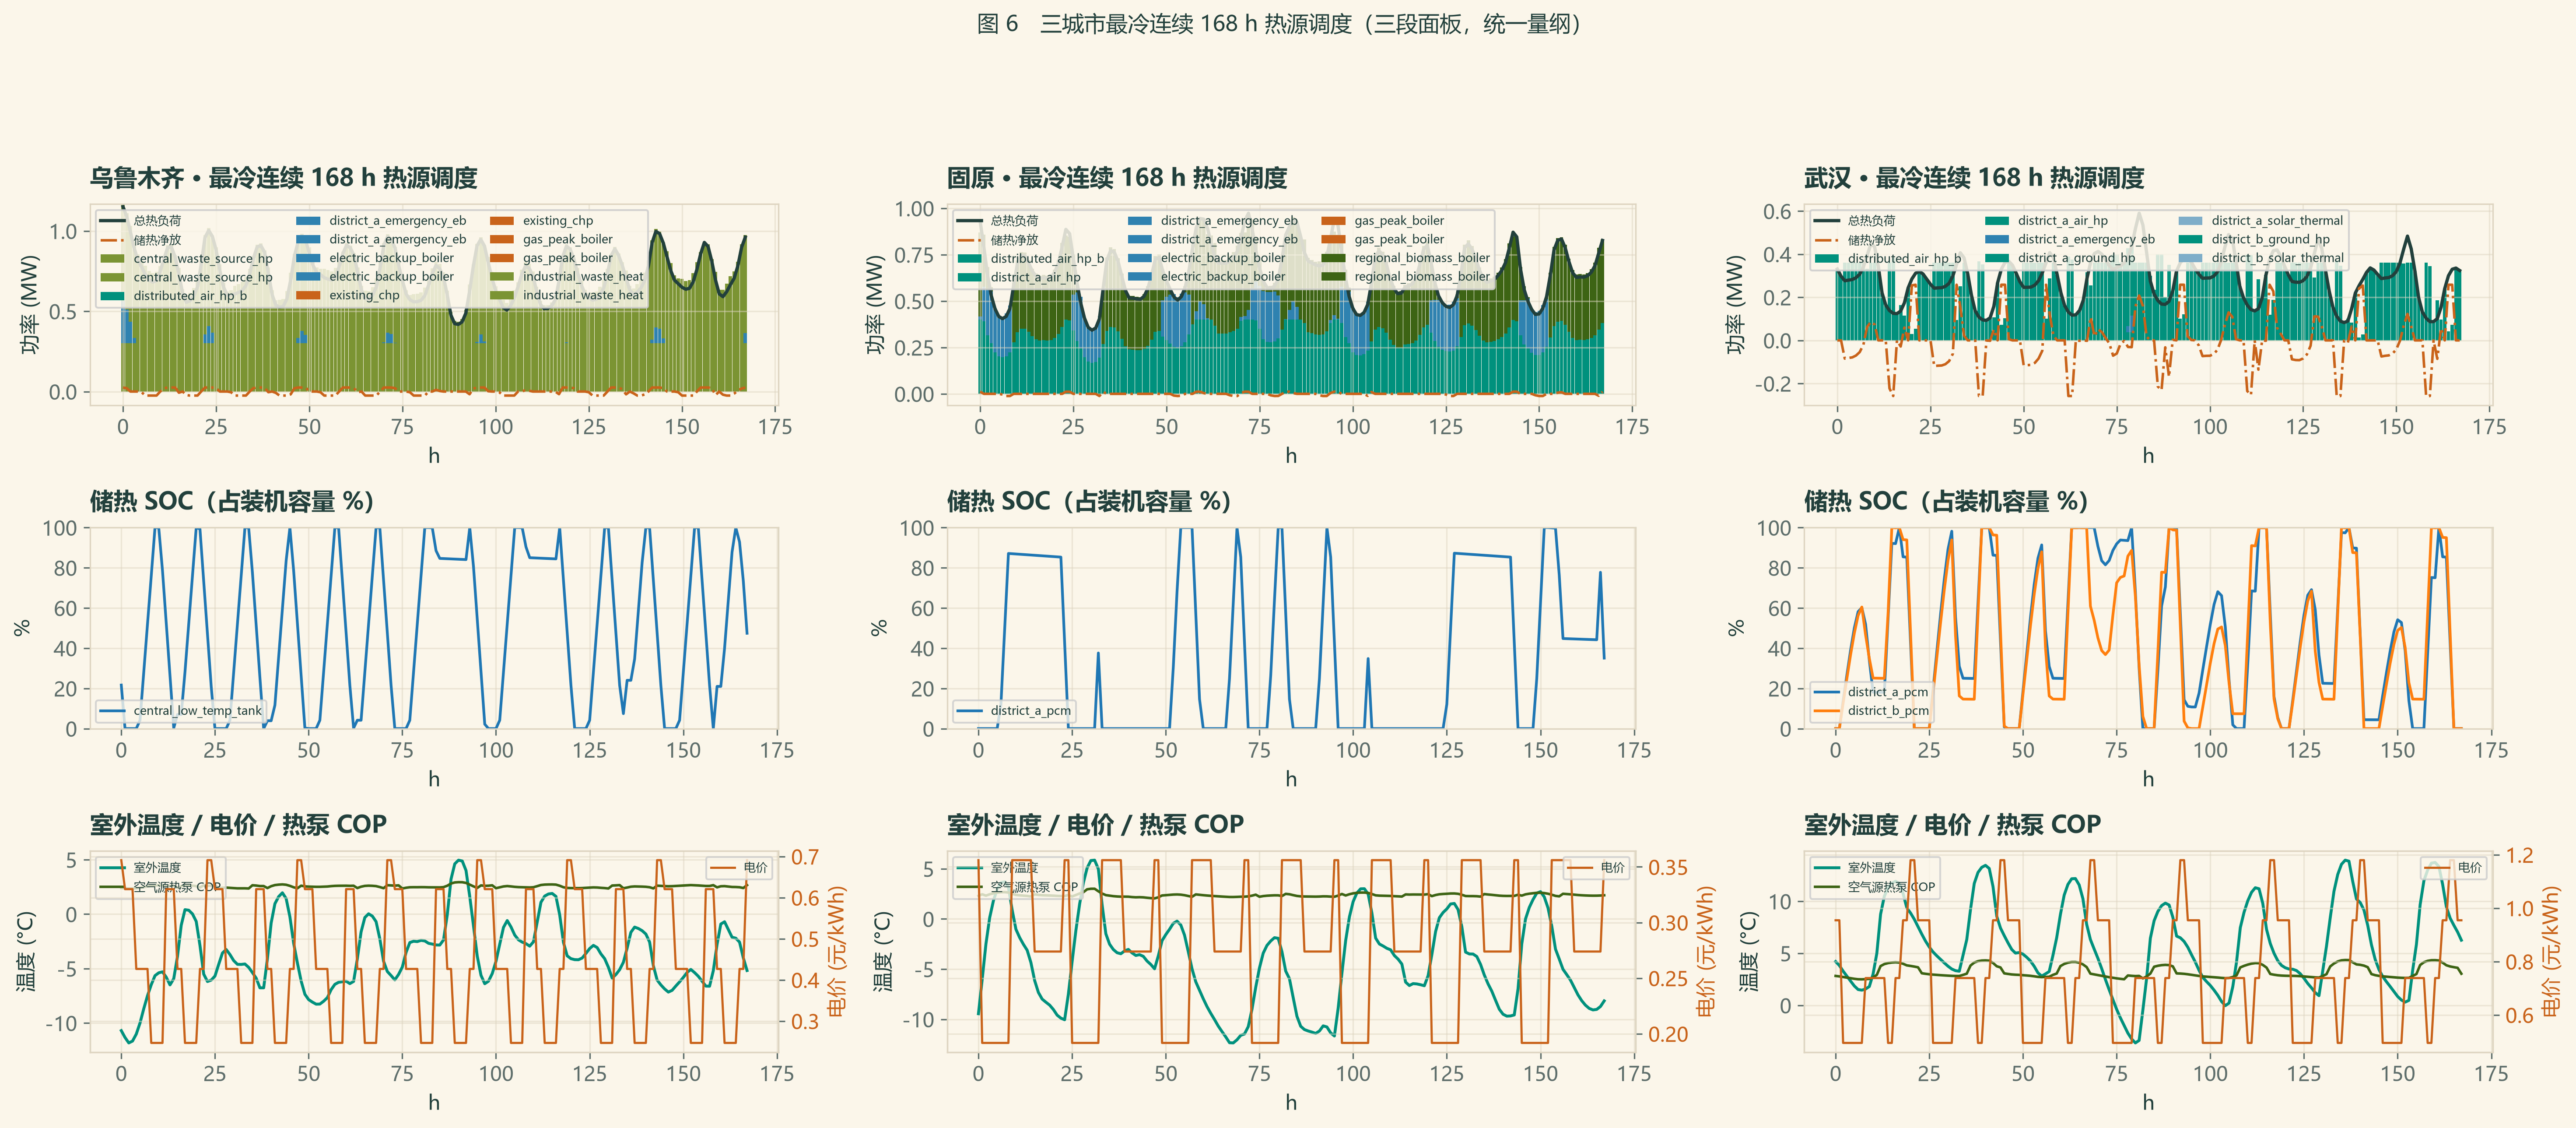
\includegraphics[width=0.98\textwidth,height=0.54\textheight,keepaspectratio,trim=0 0 0 100,clip]{media/code-results/fig06_coldest_168h_dispatch.png}
\caption{最冷连续168 h调度}
\label{fig:code-cold168}
\end{figure}

\begin{figure}[H]
\centering
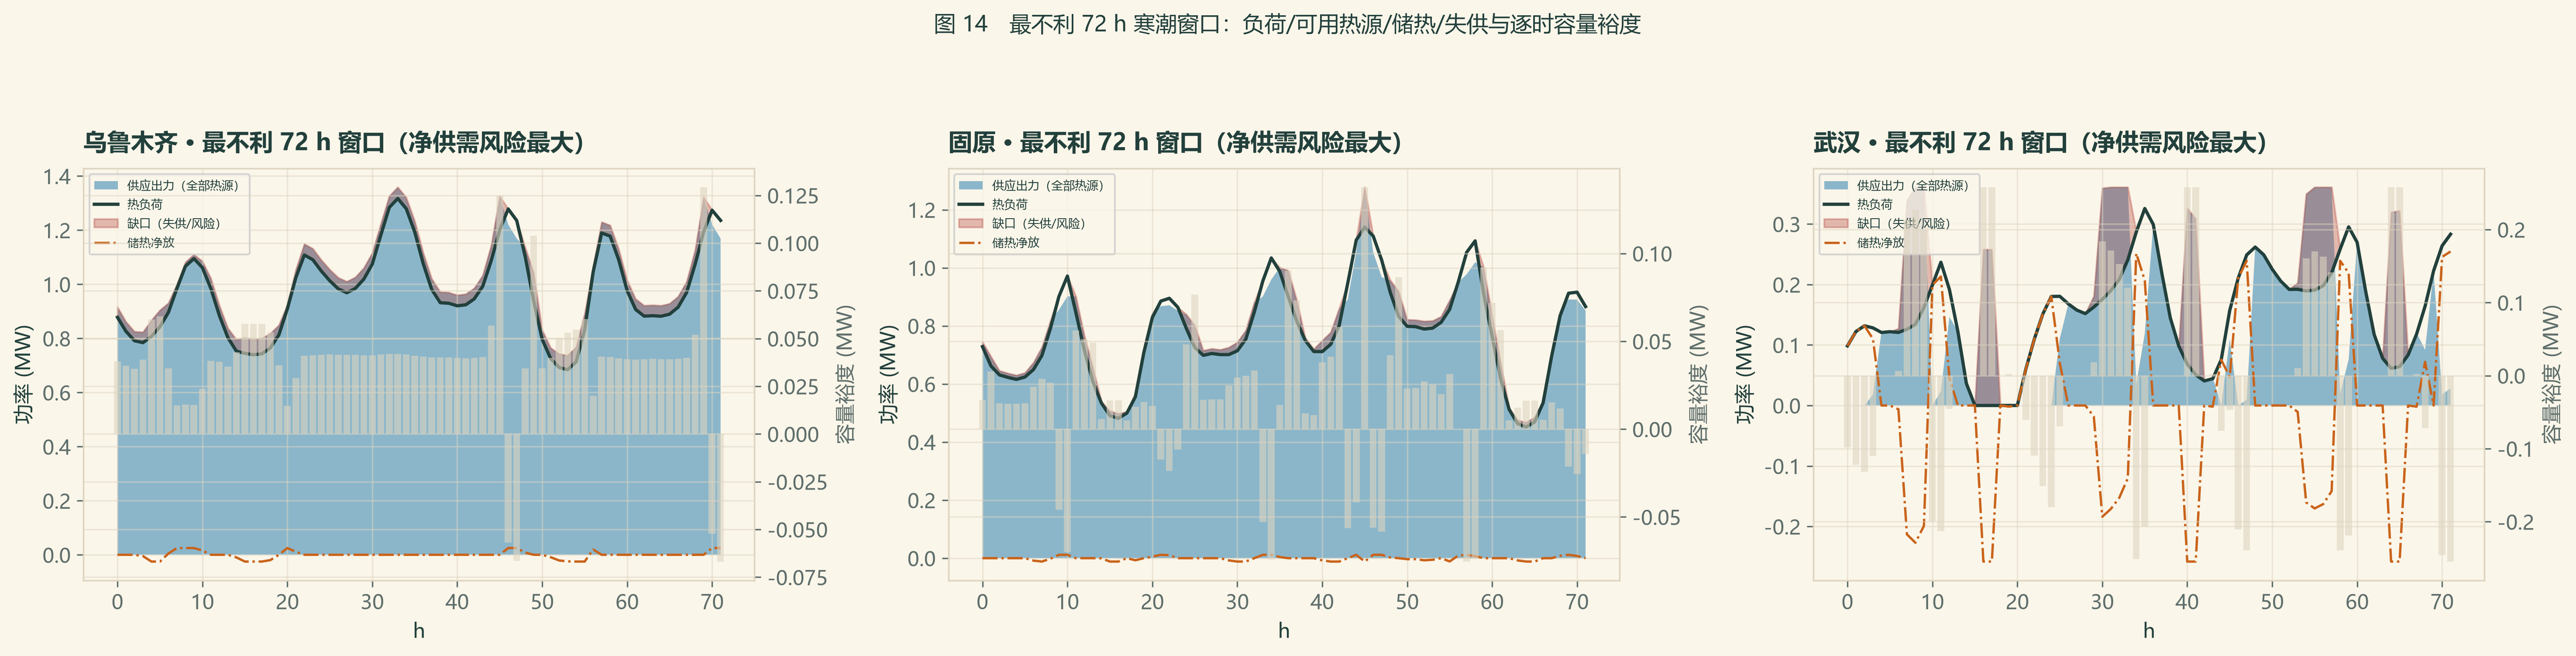
\includegraphics[width=0.98\textwidth,height=0.43\textheight,keepaspectratio,trim=0 0 0 100,clip]{media/code-results/fig14_worst_72h_resilience.png}
\caption{最不利72 h韧性窗口}
\label{fig:code-worst72}
\end{figure}

与“单年或五年聚合代表时段、最小化平均成本”的基准相比，多气象年回放使用约3---4倍代表行数，5个气象年的容量审计均通过，最差场景失供率仍为0。消融实验、压力测试和数据可靠性分级见图\ref{fig:alg-ablation}。

\begin{figure}[H]
\centering
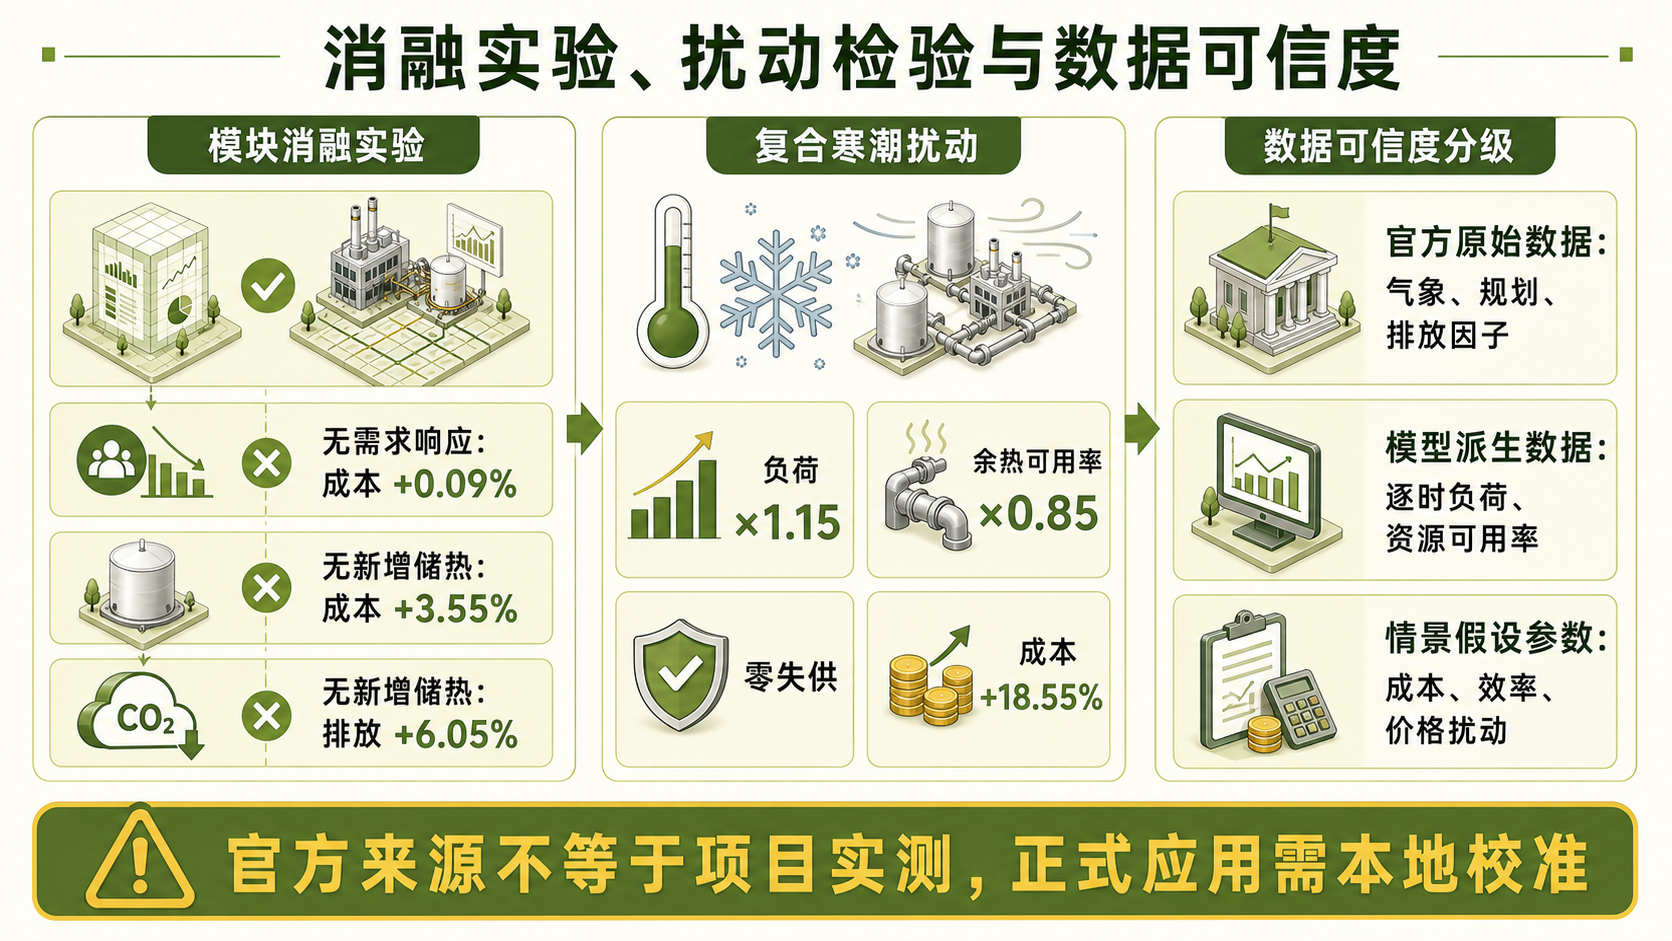
\includegraphics[width=0.76\textwidth,height=0.30\textheight,keepaspectratio]{media/algorithm-revision/fig5.png}
\caption{消融实验、扰动检验与数据可靠性}
\label{fig:alg-ablation}
\end{figure}

\subsection{数据基础与适用范围}

气象数据采用NASA POWER格点逐时数据，空间分辨率为$0.5^{\circ}\times0.625^{\circ}$，不作为地面站实测数据。标准、批复与政府文件为适用字段提供来源；派生负荷、原型热工和容量、设备成本与燃料价格按历史算例假设登记。数据记录包括来源、链接、检索时间、单位、分辨率、换算公式和适用局限。

碳排放统一采用2023年全国电力平均排放因子0.5306~kg~CO$_2$/kWh计算。新疆、宁夏和湖北的省级参考因子分别为0.6021、0.6187和0.4044~kg~CO$_2$/kWh，省级因子重算可作为地方应用时的补充。三场景均为代表性多节点系统，缩比系数仅用于规模换算，不表示对城市地理系统的完整复刻，横向比较采用单位指标。

\subsection{小结}

算法采用$\varepsilon$-约束处理成本与碳排放的多目标关系，以硬边界约束可靠性，并以$\lambda$-CVaR描述风险态度。乌鲁木齐获得投资---运行联合解；固原和武汉获得锚定投资模式下的全季运行解。三场景热平衡最大绝对残差分别为$7.41\times10^{-13}$、$1.25\times10^{-10}$和$8.53\times10^{-14}$~kW。多尺度耦合通过节点---温位聚合、建筑等效热状态递推以及城市、区域与用户层之间的共享变量实现。

原稿报告成本---碳排放二维$\varepsilon$-约束登记候选解；非支配性限于已取得且口径一致的样本。后续可进一步开展三维Pareto扩展、省级排放因子重算，以及连续温位、C\&CG、Benders分解和在线MPC等方法的计算研究。
